\documentclass[a4paper, 11pt]{article}
\usepackage{comment}
\usepackage{fullpage}
\usepackage{amsmath}
\usepackage{amssymb}
\usepackage{mathtools}
\usepackage{fontspec}
\usepackage{siunitx}
\defaultfontfeatures{Ligatures=TeX}
\usepackage{xfrac}
\usepackage{icomma}
\usepackage[section,below]{placeins}
\usepackage[labelfont=bf,font=small,width=0.9\textwidth]{caption}
\usepackage{subcaption}
\usepackage{graphicx}
\usepackage{grffile}
\usepackage{float}
\floatplacement{figure}{htbp}
\floatplacement{table}{htbp}
\usepackage{booktabs}
\usepackage{hyperref}
\begin{document}
\noindent
\centerline{\small{\textsc{Michigan State University}}} \\
\large{\textbf{CMSE/CSE 822 – Parallel Computing \hfill Fall 2019 \\
Homework 3}} \\
Alexander Harnisch \\
\noindent\makebox[\linewidth]{\rule{\textwidth}{0.4pt}}

\section*{1) Compilers and auto-vectorization}
\subsection*{a.}
\label{sec:1a}
The Intel16 system's CPU used here is a Xeon E6-2680 by Intel, running at a
clock speed of \SI{2.4}{\giga\hertz}. Figure~\ref{fig:cache_table} shows the
cache size and layout. However, the processor supports turbo boosting at
\SI{3.3}{\giga\hertz} for a single core and \SI{2.9}{\giga\hertz} for all 14
cores at once. The CPU has 14 physical cores with Intel's hyper-threading
technology, effectively having 24 virtual cores or simultaneous threads.
Assuming the processor is capable of one floating point operation per clock
cycle and thread running at \SI{2.9}{\giga\hertz} turbo boost, the theoretical
peak performance would be \SI{96.6}{\giga FLOP \per\second}. However, the
assignment is not precise enough to know what exactly it is asking for. Single
thread performance? Turbo boost yes or no? The theoretical single thread peak
performance at a boosted clock frequency of \SI{3.3}{\giga\hertz} would simply
be \SI{3.3}{\giga FLOP\per\second}. The sustainable single thread peak
performance at \SI{2.4}{\giga\hertz} would be \SI{2.4}{\giga FLOP\per\second}.
Multiply that by 24 for sustainable multithread peak performance. 
\begin{figure}
  \centering
  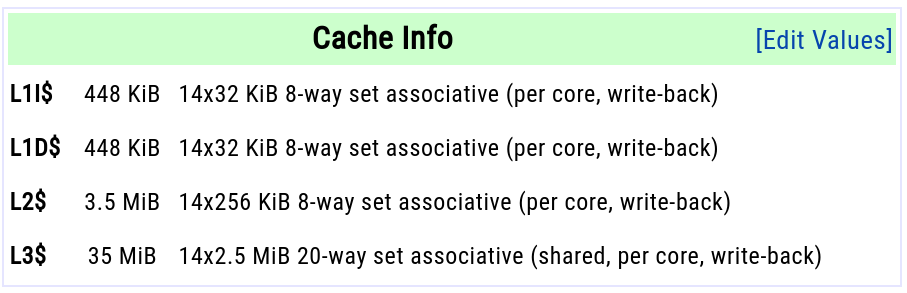
\includegraphics[width=.7\textwidth]{./cache_table.png}
  \caption{Xeon E5-2680 v4 cache size and layout~\cite{wikichip}.}
  \label{fig:cache_table}
\end{figure}

\subsection*{b.}
This depends on many assumptions that have to be made and are not given by
the problem statement. Assuming \SI{32}{bit} single-precision floating point
numbers, AVX can perform the same instructions on up to 8 data streams at a
time. Four at a time for double precision. That would mean we get another
factor of 8 or 4. Additionally, assuming that all operations are of the type
$a+b\times c$ which can be done in one operation using FMA we get another
factor of 2.

\subsection*{c.}
The plot using GCC is given by Figure~\ref{fig:1_gcc}. Figure~\ref{fig:1_icc}
shows the results using the Intel compiler.
\begin{figure}
  \centering
  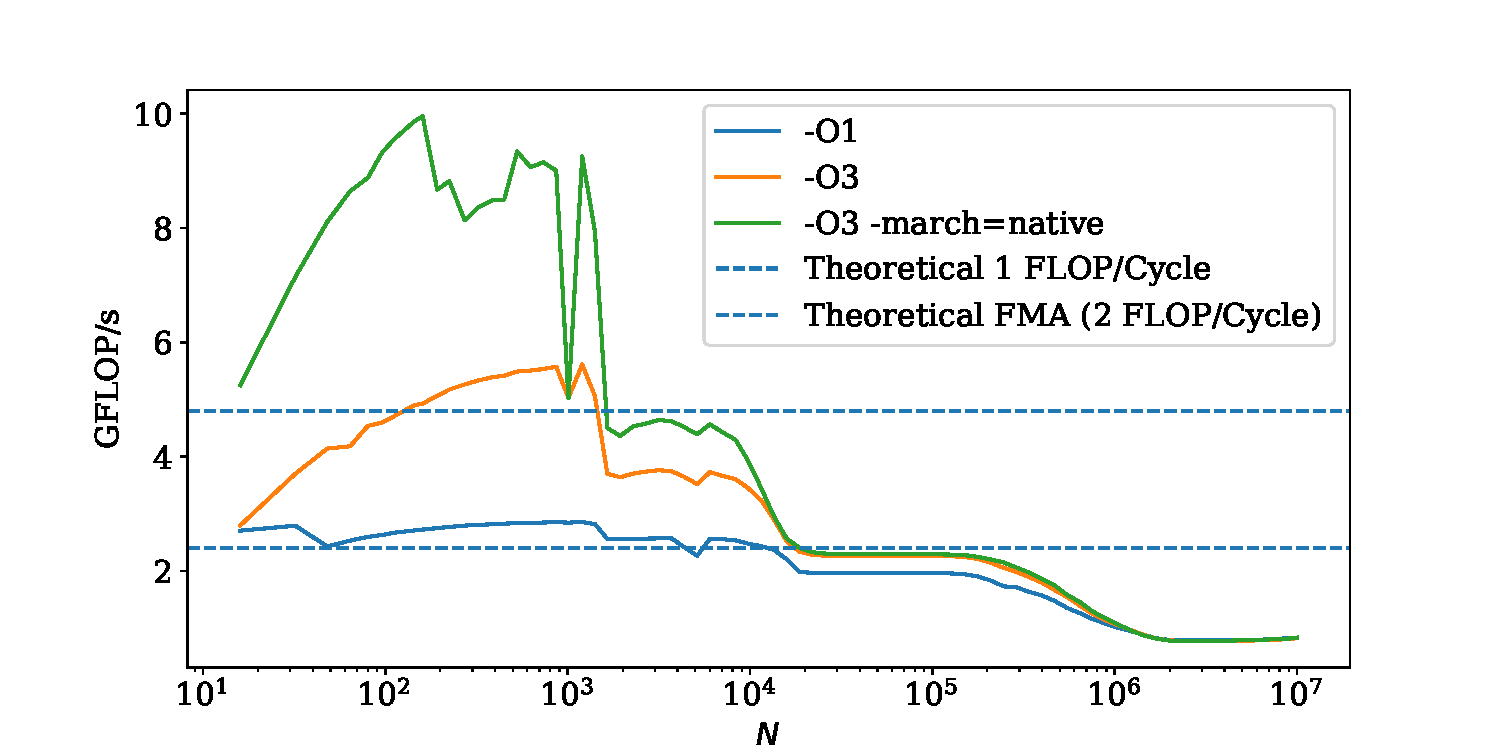
\includegraphics[width=\textwidth]{../plot/1/1b_gcc.pdf}
  \caption{Performance of the vector triad kernel using different compiler
  settings for the gcc compiler.}
  \label{fig:1_gcc}
\end{figure}
\begin{figure}
  \centering
  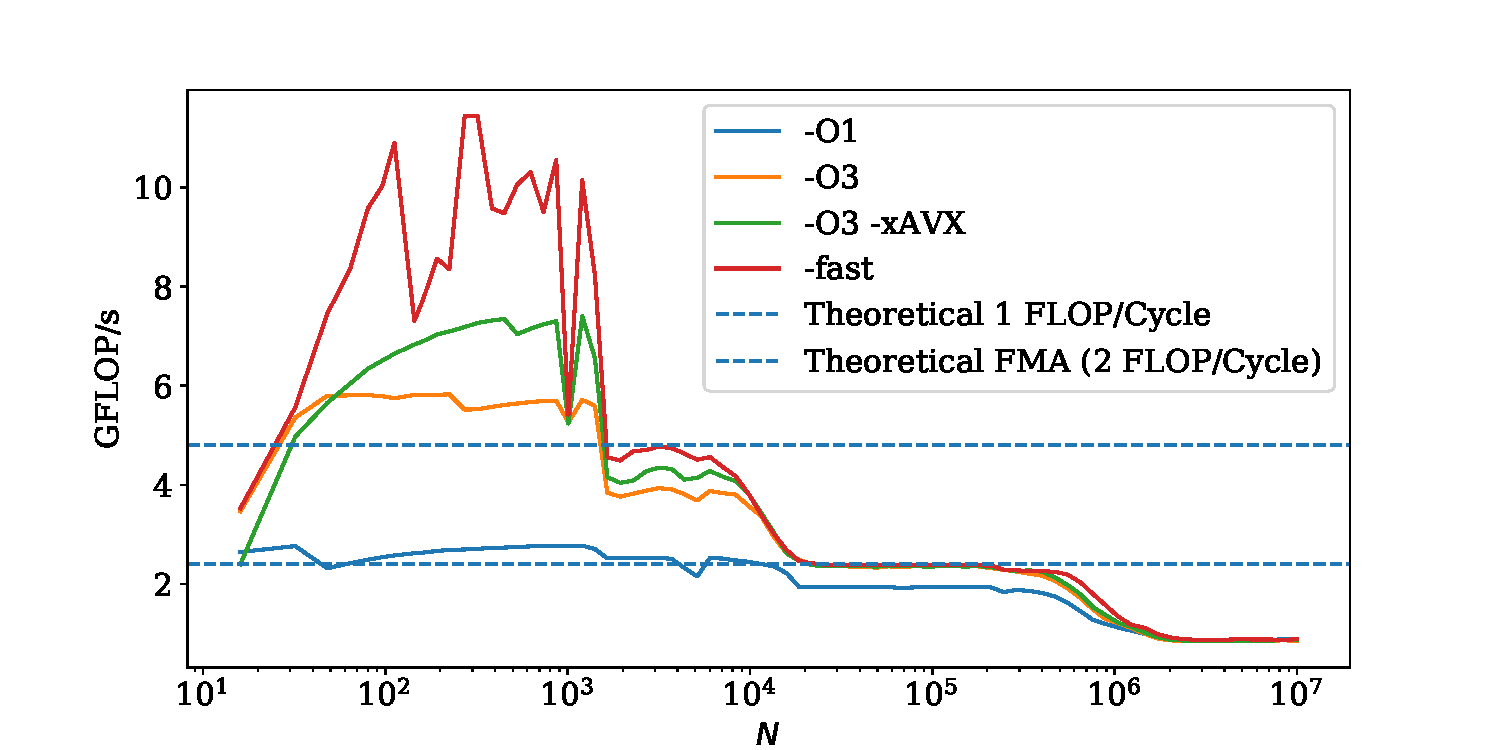
\includegraphics[width=\textwidth]{../plot/1/1b_icc.pdf}
  \caption{Performance of the vector triad kernel using different compiler
  settings for the Intel compiler.}
  \label{fig:1_icc}
\end{figure}

\subsection*{d.}
It seems like the O3 flag enables FMA. With only O1 the measured performance
more or less consistently hovers around the expected peak performance assuming
1 FLOP per cycle. For small $N$ that make perfect use of the L1 cache, the
results are inconclusive. They do not reach the theoretical peak performance. 

\subsection*{e.}
There is a clear step structure in both plots, caused by the cache structure.
The steps occur exactly where the corresponding cache level is used up
according to Figure~\ref{fig:cache_table}, since $N\cdot\SI{8}{byte}$ is
roughly the amount of fast memory used.

\section*{2) Stream benchmark and memory bandwidth}
\subsection*{a.}
The bandwidths reported by STREAM are shown in Table~\ref{tab:stream}.
\begin{table}
  \centering
  \begin{tabular}{lllll}
    Function  &Best Rate MB/s &   Avg time  &   Min time  &  Max time \\
    \hline 
    Copy:     &      10718.2  &   0.150111  &   0.149278  &   0.152882 \\
    Scale:    &      11116.3  &   0.144151  &   0.143933  &   0.144601 \\
    Add:      &      11912.0  &   0.202684  &   0.201477  &   0.209135 \\
    Triad:    &      11863.3  &   0.202537  &   0.202304  &   0.202677 \\
  \end{tabular}
  \caption{STREAM output for $N=10^{8}$.}
  \label{tab:stream}
\end{table}

\subsection*{b.}
The memory bandwidth varies depending on the compiler and settings. See next
section.

\subsection*{c.}
The results are shown in Figure~\ref{fig:2_gcc} and Figure~\ref{fig:2_icc}.
\begin{figure}
  \centering
  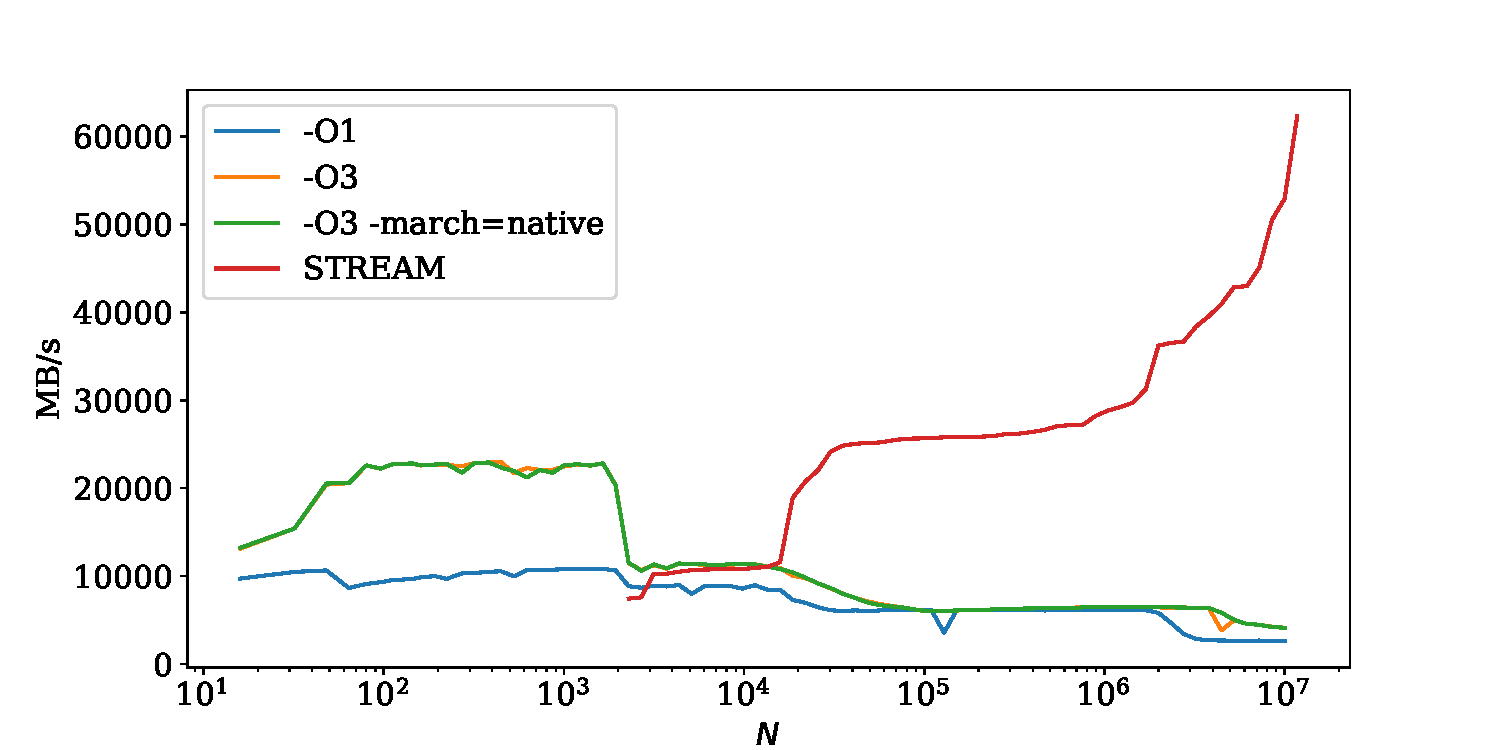
\includegraphics[width=\textwidth]{../plot/2/gcc.pdf}
  \caption{Results using the gcc compiler.}
  \label{fig:2_gcc}
\end{figure}
\begin{figure}
  \centering
  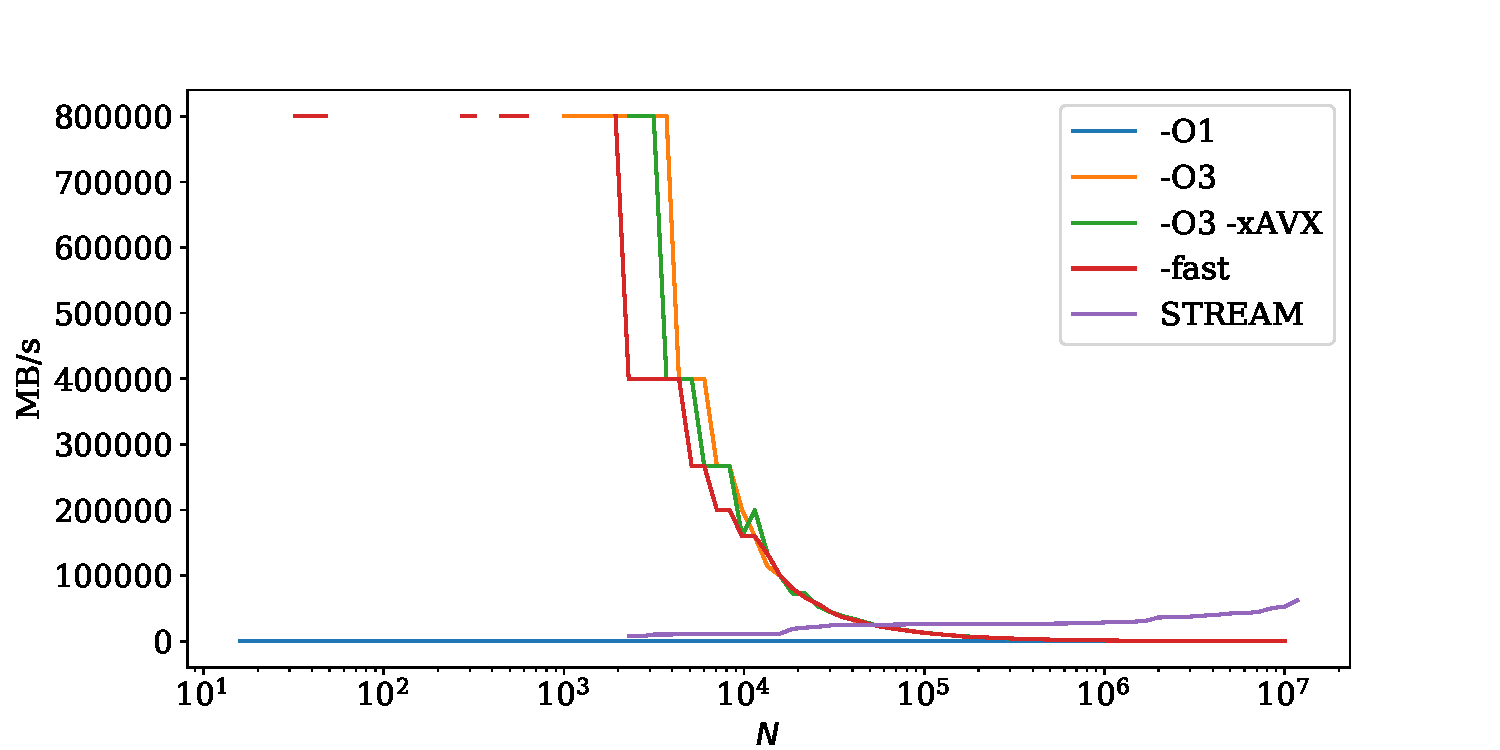
\includegraphics[width=\textwidth]{../plot/2/icc.pdf}
  \caption{Results using the Intel compiler.}
  \label{fig:2_icc}
\end{figure}

\subsection*{d.}
We can barely measure the bandwidth for small $N$, where the L1 cache is big
enough the hold all data. In the L2 are, the STREAM result and gcc result are
in agreement. However, for larger $N$ the simple vector copy code
underperforms.

For some reason the time measurement seems to be less accurate when using the
Intel compiler, even though for both figures I did use the exact same source
code. It seems like for small $N$ the time is just so small that it can not be
measured accurately.

I'm sad that the results are inconclusive, I put a lot of time into it but just
don't have more time for this assignment.

%%%%%%%%%%%%%%%%%%%%%%%%%%%%%%%%% Bibliography %%%%%%%%%%%%%%%%%%%%%%%%%%%%%%%%
\begin{thebibliography}{9}
  \bibitem{wikichip}
  WikiChip.
  \textit{Xeon E5-2680 v4 - Intel}.
  \href{https://en.wikichip.org/wiki/intel/xeon\_e5/e5-2680\_v4}
  {https://en.wikichip.org/wiki/intel/xeon\_e5/e5-2680\_v4}.
\end{thebibliography}
\end{document}
